\documentclass[a4paper]{jpconf}

%% Packages
\usepackage[pdftex]{graphicx}
\usepackage{color}
\usepackage{subfig}
\usepackage{amssymb}
\usepackage{amsmath}
\usepackage{placeins}
%\usepackage{subfigure}
%\usepackage[margin=10pt,font=small,labelfont=bf]{caption}
%\usepackage{subcaption}

%% Notation macros
\newcommand{\G}{\mathcal{G}}
\newcommand{\Gbar}{\bar{\mathcal{G}}}

%% editing macros
\newcommand{\red}[1]{{\color{red}#1}}
\newcommand{\ira}[1]{\red{(#1 --Ira)}}

\begin{document}

%% Title block
\title{LISA Pathfinder as a Micrometeoroid Instrument}

% jpconf class is *incompatible* with authblk package. have to do it the old-fashioned way! 
% Author list (need to check if this author list has changed since LISA X)
\author{
J.I.~Thorpe$^{a}$,
T.B. ~Littenberg$^{b}$,
J. ~Baker$^{a}$,
and J.~Slutsky$^{a}$,
for the The LISA Pathfinder Team
}
\address{$^{s}$ NASA Goddard Space Flight Center, 8800 Greenbelt Road, Greenbelt, MD 20771, USA}
\address{$^{u}$ NASA Marshall Space Flight Center, Redstone Arsenal, Huntsville, AL 35812, USA}


\ead{james.i.thorpe@nasa.gov}

%% Abstract
\begin{abstract}
LISA Pathfinder is perhaps the most precise accelerometry instrument ever flown in space. The drag-free control system can sense and react to external disturbances of an extremely small magnitude. One class of such disturbances are the impacts of micrometeoroids or dust. A simple model of the LPF system suggests that individual impacts with transferred momentum exceeding a few tens of nanoNewton-meters are detectable. Furthermore, the ability of LPF to resolve both the linear and angular momentum transfer as vector quantities allows information such as the sky location and the impact location of the impactor to be reconstructed. This novel approach to micrometeoroid detection and characterization, as well as the location of LPF at L1, provide an opportunity to improve our understanding of the dust environment in the inner solar system. Here we present some preliminary findings from LPF, including four candidate impact events.
\end{abstract}

%% INTRO
\section{Introduction}
\label{sec:intro}
LISA Pathfinder (LPF) \cite{LPF_LISAX}is a technology demonstrator mission for future space-based gravitational wave observatories. Led by the European Space Agency and with contributions from a consortium of European member states and NASA, the mission was launched on December 3rd, 2015 and began science operations on March 1st, 2016. The operational orbit is a $0.8\,\textrm{Mkm} \times 0.5\,\textrm{Mkm}$ Lissajous orbit around the first Earth-Sun Lagrange point (L1), a gravitational balance point that lies approximately $1.5\,\textrm{Mkm}$ in the sunward direction from Earth. LPF has been operating in a variety of modes through baseline operations of its European payload (March-June 2016), baseline operations of its NASA payload (July-November 2016), and extended mission operations (December 2016 - present).
\par
The primary purpose of these operations is to demonstrate drag-free control as a technique for producing a low-disturbance inertial reference that could be used as the basis for a long-baseline gravitational wave observatory. In LPF, the reference is a $4\,\textrm{cm}$ cube of Au-Pt alloy with a mass of approximately $1.92\,\textrm{kg}$. This `test mass' is contained within an electrode housing that is fixed to the spacecraft that can be used to both measure the position and attitude of the test mass relative to the spacecraft as well as to apply forces and torques between the test mass and spacecraft. A control system maintains gaps between the spacecraft and test mass by monitoring the separation and applying force or torque commands to the test mass via the electrode housing or to the spacecraft via a micropropulsion system. In typical drag-free operations the spacecraft is commanded to follow the test mass in one axis (denoted as $x$) and the test mass is forced to follow the spacecraft in other degrees-of-freedom (DoF). Additionally, an interferometric metrology system is employed to measure the relative separation between the test mass and spacecraft along the $x-$axis with sub-picometer precision and rotations along the $y-$axis and $z-$axis with nanoradian precision.
\par
LPF carries a second test mass, located approximately $38\,\textrm{cm}$ from the primary test mass in the $x$ direction. This test mass is used as a witness to characterize the residual disturbances of the drag-free test mass. This differential acceleration measurement has the advantage that it common-mode rejects external disturbances on the spacecraft, such as fluctuations in the solar radiation pressure, solar wind, magnetic environment, and particle impacts. This strategy is effective for characterizing drag-free test masses as references for gravitational-wave instruments and was successfully employed to demonstrate residual acceleration noise significantly below the LPF mission requirements and consistent with levels required for LISA-like gravitational wave observatories \cite{LPF_PRL}.
\par
In addition to this primary science goal, the external disturbances present in the single-test mass signal represent an opportunity to characterize the space environment of LPF in a unique and novel way - by measuring acceleration of the spacecraft. In a previous work \cite{Thorpe2016} it was shown that impacts of dust and micrometeoroids should be detectable in LPF if they transferred momentum to the satellite of a few tens of $\mu\textrm{N}\cdot\textrm{s}$. It was estimated that such events should occur relatively frequently and that LPF should be able to measure properties including the total transferred momentum, momentum direction, and location of impact on the spacecraft.  In this paper we present four impact candidates from the operations period of March 1, 2016 through June 28, 2016.  This does not represent a complete catalog during this time period but rather an example of typical events. 
\par
In section \ref{sec:recon}, we present one event and describe the process of reconstructing the external force from the measured positions and attitudes of and the commanded forces and torques. In section \ref{sec:models} we describe the 6-DoF model used to fit the impact candidates. In section \ref{sec:results} we present the four impact candidates and the model fits. Section \ref{sec:discuss} summarizes our results and describes ongoing and future work with this data set.

\section{Event Reconstruction}
\label{sec:recon}
The goal of the reconstruction process is to remove the effect of the LPF control loops and estimate the dynamics of the spacecraft and test mass as if they were kinematicly free bodies. The signals available for this are the measured position and attitude of the test mass (6 DoFs from electrostatic measurements, 3 DoFs from interferometry), the commanded force and torque to the spacecraft, and the commanded force and torque to the test mass. The reconstruction is done in the acceleration domain to avoid integration constants that do not contribute to the micrometeoroid signal. For example, in the $x$-axis, in which the spacecraft test mass separation is controlled by forcing the spacecraft, the external spacecraft acceleration can be estimated using the following equation:
\begin{equation}
a_{ext}(t) = \frac{d^2x(t)}{d t^2} - \frac{1}{M}C\,F(t-\tau) - \omega^2 x(t),\label{eq:x_recon}
\end{equation}
where $a_{ext}(t)$ is the external acceleration, $x(t)$ is the measured position, $F(t)$ is the commanded force, $M$ is the spacecraft mass, C is the gain in the micropropulsion system,  $\tau$ is a delay in the response of the micropropulsion system, and $\omega^2$ is a term describing the ``stiffness'', a spring-like coupling between the test mass and spacecraft that arises from electrostatic, magnetic, and gravitational effects. Quantities such as $C$, $\tau$, and $\omega^2$ are measured using signal injections as part of the normal LPF measurement campaign.

Figure 1 shows an example of an impact candidate and the reconstructed external acceleration in the $x$-axis. In the top panel of Figure \ref{fig:posForce}, the position of the test mass relative to the spacecraft exhibits a sharp rise that is indicative of an impact. The bottom panel of Figure \ref{fig:posForce} shows the corresponding force command, which includes the control system's response to this disturbance. The control system does its job of rejecting the disturbance and settles into steady-state after one or two oscillations. Figure \ref{fig:extForce} shows the reconstructed external acceleration, which is an approximate delta function, as would be expected for an impact. A slight overshoot is believed to be a reconstruction error associated with inaccuracies in the parameters used in (\ref{eq:x_recon}) or interpolation errors when applying sub-sample delays. 

\begin{figure}[h!]
	\centering
	\subfloat[SC position and Force\label{fig:posForce}]{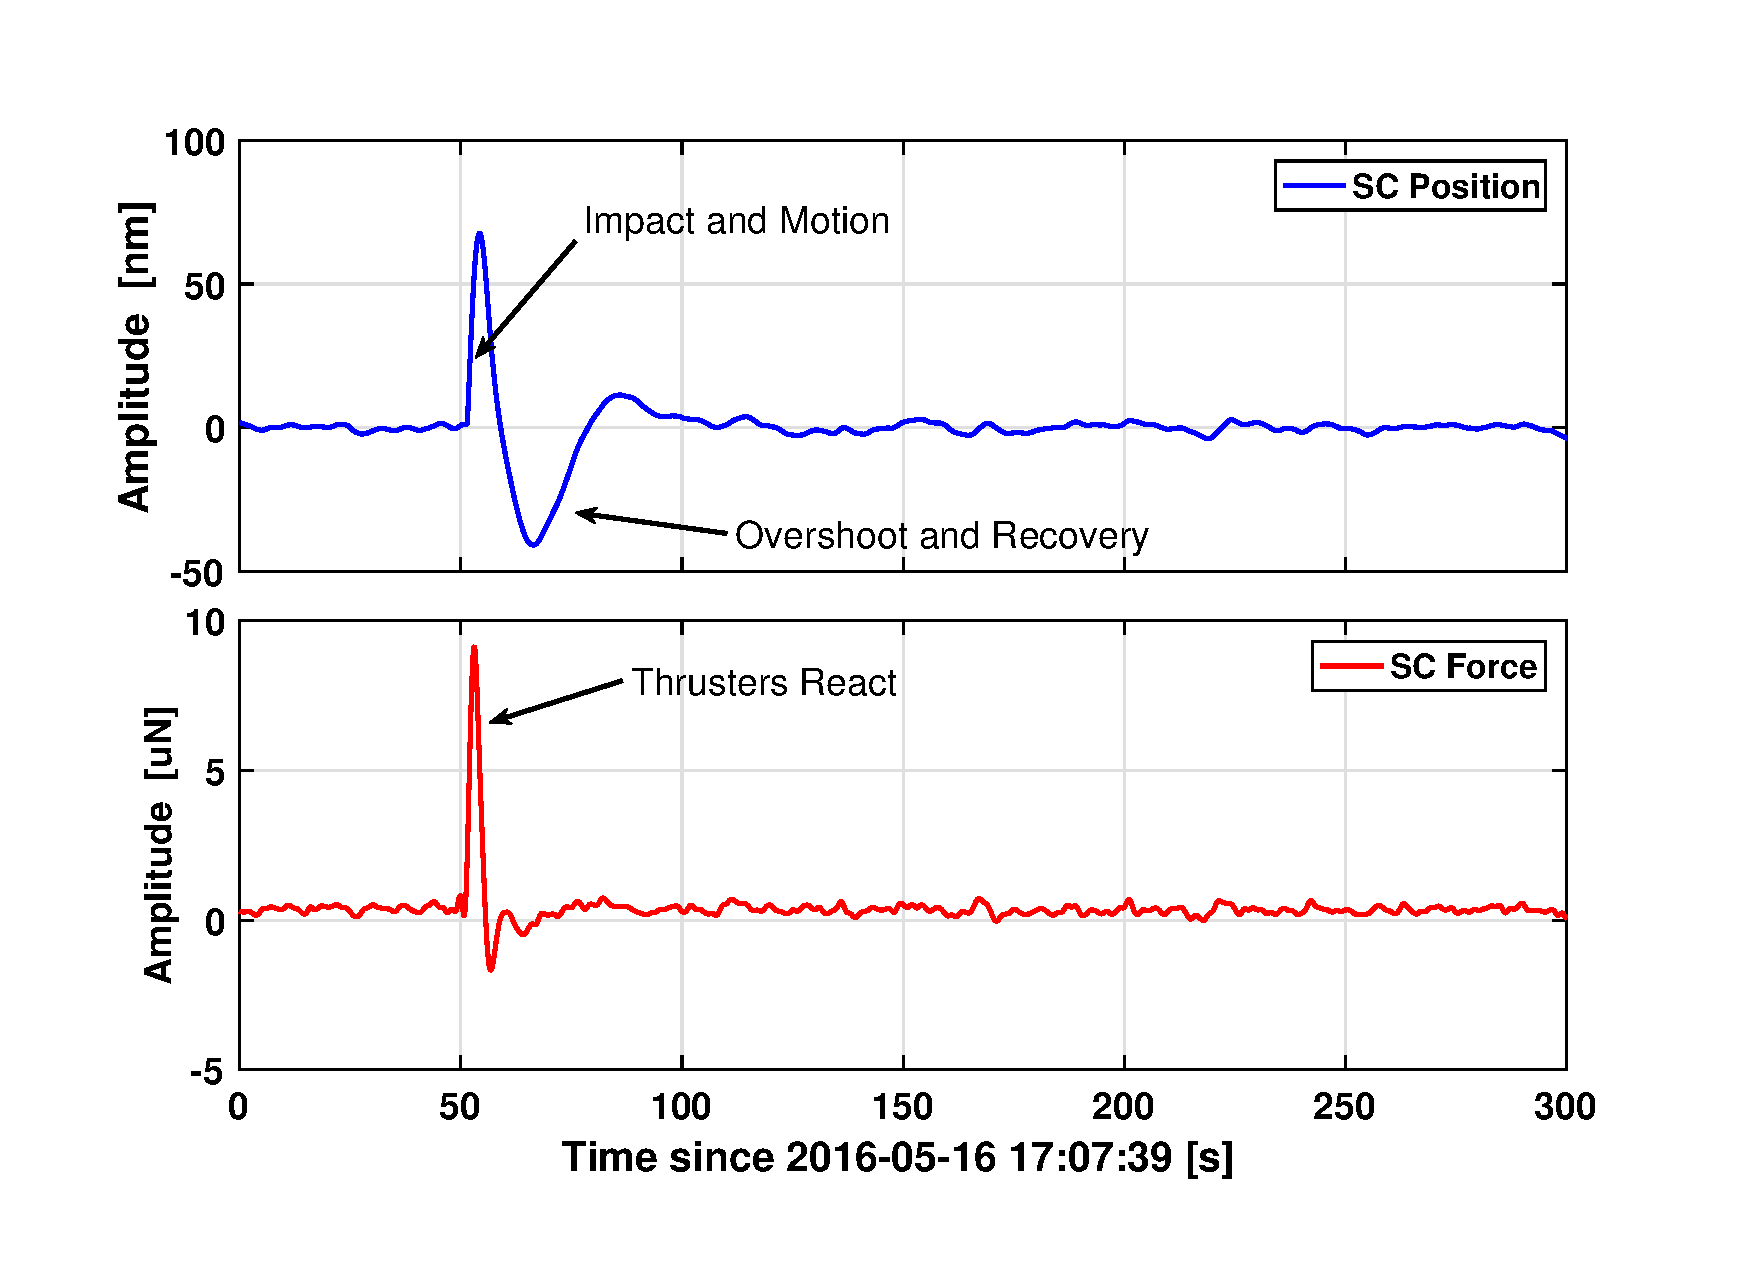
\includegraphics[width=7 cm]{figures/Figure1a.eps}}\quad
	\subfloat[Reconstructed External Force\label{fig:extForce}]{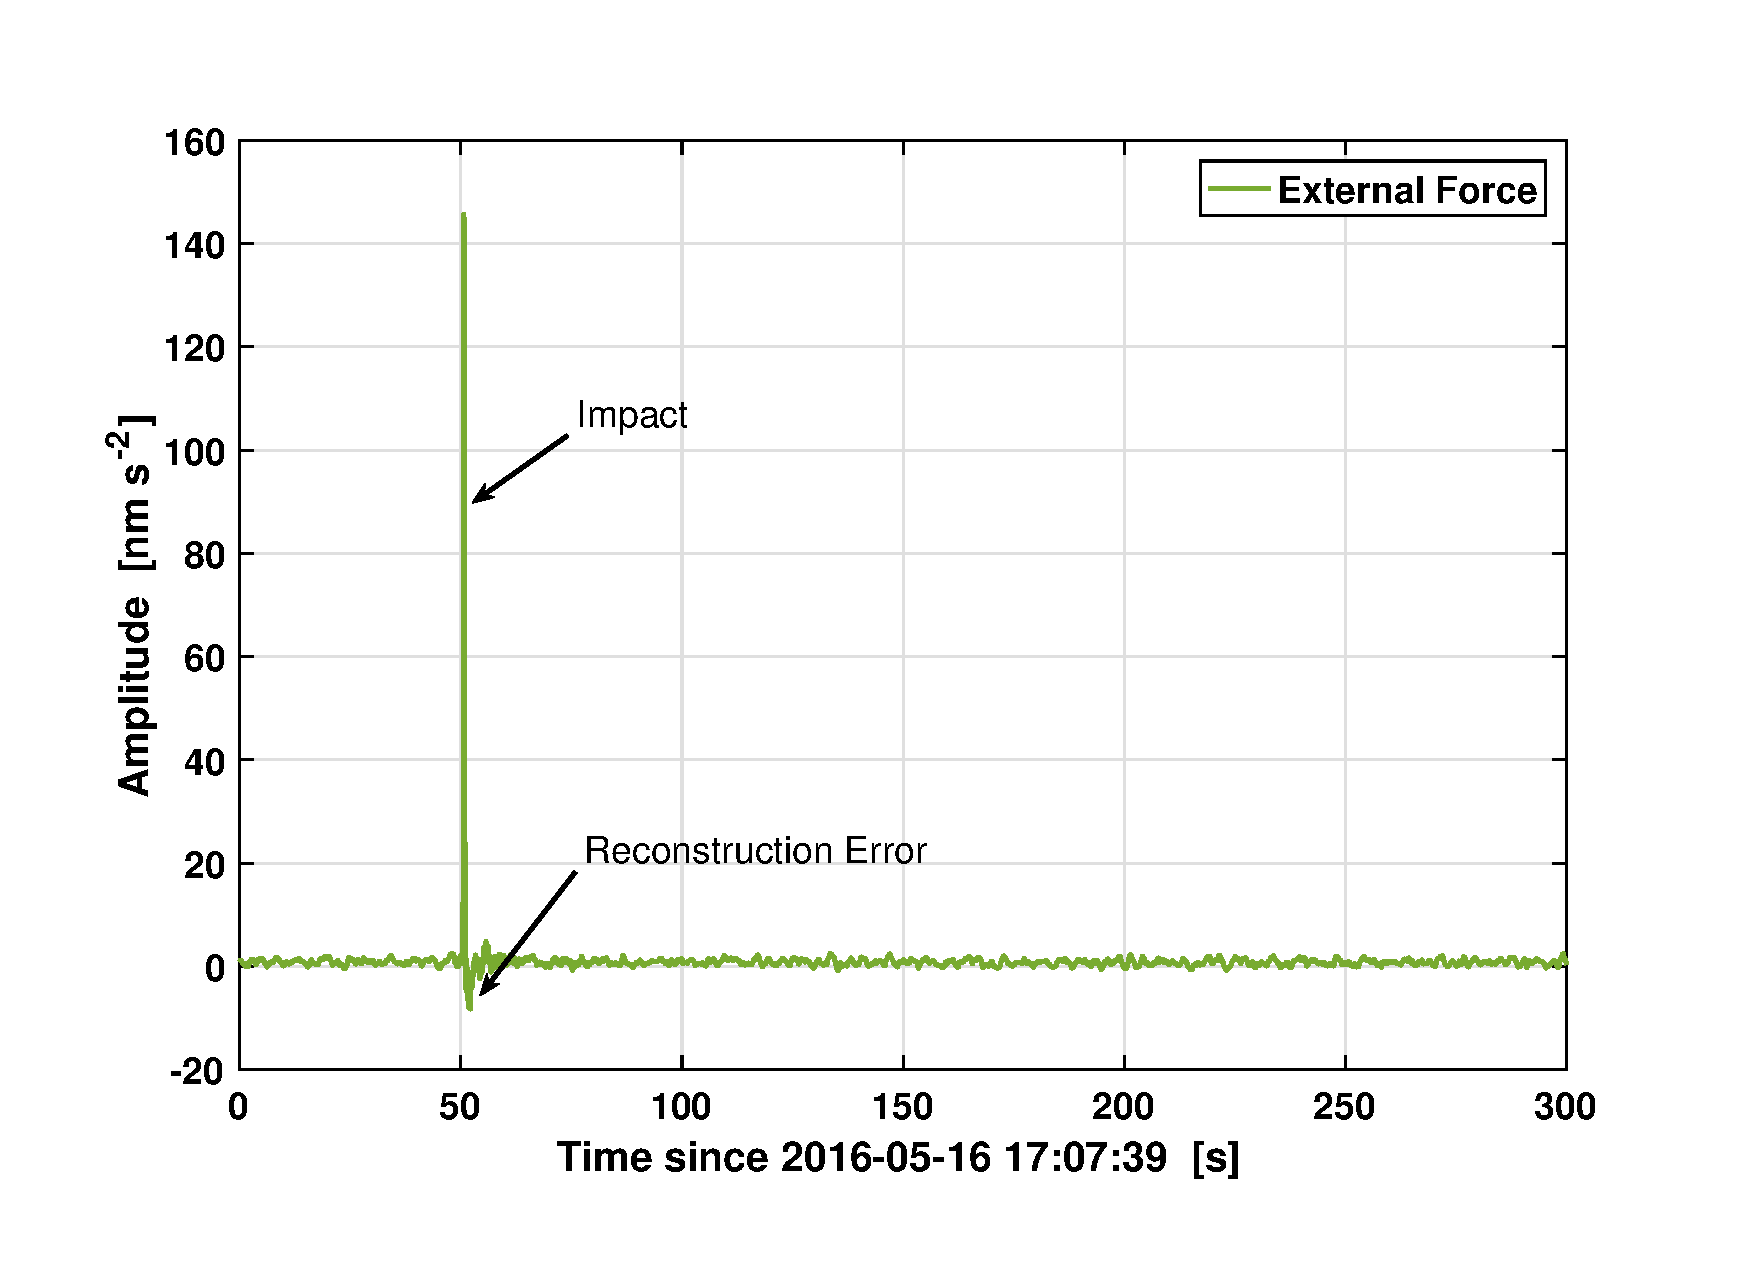
\includegraphics[width=7 cm]{figures/Figure1b.eps}}\\	
	\caption{x-axis dynamics for a candidate impact event. Left panel top shows relative motion of test mass and spacecraft along x as measured by the interferometer. Left panel bottom shows force commanded by drag-free system to the spacecraft along x. Right panel shows external force along x as reconstructed from the measured position, commanded force, and knowledge of the spacecraft mass and stiffness.}
\end{figure}

When extending this reconstruction process to all six DoFs, care must be taken to account for couplings between the linear and angular DoFs as measured by the test masses, which are offset from the spacecraft center of mass in both the $+z$ direction and along the $x$-axis. To address this coupling, the applied forces and torques on the spacecraft are first used to estimate the linear and angular acceleration in the spacecraft body frame (a cartesian frame with the origin at the spacecraft the center of mass). These accelerations are then used to compute the contribution to the acceleration at the test masses using the known location of the housings relative to the spacecraft body frame.

\section{Models}
\label{sec:models}
To identify impact candidates and estimate the parameters of interest, a model of the system's response is needed. Since the event reconstruction described in Section \ref{sec:recon} produces the equivalent acceleration of the spacecraft as a free body, the impact model only needs to account for the 3D kinematics of the spacecraft. The impact model assumes that the impact timescale is short relative to the sample cadence of the LPF data (typically $0.1\,\textrm{s}$) such that the impact can be represented as a delta-function in acceleration. The geometric coupling of the impact momentum to different DoFs is identical to that for the micropropulsion system and is computed in two steps. First, the acceleration in the body frame is computed for both linear and angular DoFs:
\begin{eqnarray}
\vec{a}_{x,B}(t) = P\:M^{-1}\delta(t-\tau) \hat{e},\label{eq:axB} \\
\vec{a}_{\theta}(t)= P\:\mathbf{I}^{-1}\delta(t-\tau)\left(\vec{r}\times\hat{e}\right), \label{eq:aq}
\end{eqnarray}
where $\vec{a}_{x,B}$ is the acceleration of the spacecraft body frame in the linear DoFs, $\vec{a}_{\theta,B}$ is the acceleration of the spacecraft body frame in the angular DoFs, $P$ is the total transferred momentum, $\tau$ is the impact time, $\hat{e}$ is the unit-vector in the direction of the transferred momentum, $M$ is the mass of the spacecraft, $\mathbf{I}$ is the spacecraft moment of inertia, and $\vec{r}$ is the location of the impact relative to the center of mass. The angular accelerations at the housing frame are the same as described in (\ref{eq:aq}) but the linear accelerations pick up an additional term due to the offset of the test mass from the center of mass:
\begin{equation}
\vec{a}_{x,TM}(t) = \vec{a}_{x,B} + \left(\vec{r}_{TM}\times \vec{a}_{\theta}\right),\label{eq:axTM}
\end{equation}
where $\vec{a}_{x,TM}$ is the acceleration in the linear DoFs as measured in the test mass frame and $\vec{r}_{TM}$ is the location of the test mass in the body frame.

\section{Results}
\label{sec:results}

The impact model in Section \ref{sec:models} was used in a Markov-Chain Monte-Carlo tool to both search for and characterize potential impacts in stretches of LPF data~\cite{Cornish15,Littenberg15}. Sections of data with no known signal injections were identified and passed through the event reconstruction pipeline described in Section \ref{sec:recon}.  The output of this pipeline was then divided into segments $1638.4\,$s in length and passed to the MCMC tool, which used frequency-domain versions of the models in (\ref{eq:axB}) - (\ref{eq:axTM}) to fit for the parameters $P$, $\tau$, $\hat{e}$ (represented by two sky angles), and $\vec{r}$. The impact location was constrained to lie of the surface of the spacecraft and also to be consistent with the measured sky angle (e.g. the impact location must have an unobstructed view of the origin of the momentum vector). For segments with an identified candidate, the MCMC was allowed to run for $10^5$ iterations, including a burn-in period of $10^4$ iterations.
\par

While the results of a systematic search will be the subject of a future publication, here we present four impact event candidates that occurred in the timeframe March 1, 2016 through June 28, 2016. Table \ref{tab:candidates} summarizes the recovered parameters for these events. Figure \ref{fig:amps} contains posterior distribution functions for the transferred momenta, Figures \ref{fig:sky1} - \ref{fig:sky4} show sky maps of the transferred momentum vector's origin (direction opposite to the transferred momentum), and Figure \ref{fig:loc1} - \ref{fig:loc4} show scatter plots of the MCMC samples of the recovered impact location on the spacecraft colored by the natural log of the likelihood.

\begin{table}[h!]
\caption{\label{tab:candidates}Sample impact event candidates from the first portion of LTP operations. Values represent the median of the posterior distribution and intervals represent the upper and lower limits of the $90\%$ confidence intervals. Colatitude represents the angle of the impact vector from the $+z$ direction. Azimuth represents the angle in the $x-y$ plane from the $+x$ axis.}
\begin{center}
\begin{tabular}{|c|c|c|c|c|}
\hline
Day & GPS Time $\left[\textrm{s}\right]$ & Amplitude $\left[\mu\textrm{N}\cdot\textrm{s}\right]$ & colatitiude $\left[\textrm{rad}\right]$ & azimuth $\left[\textrm{rad}\right]$ \\
\hline
 2016-04-09 & $1144229907.61^{+0.001}_{-0.0003}$ & $495^{+10}_{-9}$ & $1.576^{+0.003}_{-0.002}$ & $0.002^{+0.15}_{-0.12}$ \\
  2016-05-04 & $1146429821.79^{+0.04}_{-0.03}$ & $55^{+44}_{-23}$ & $1.60^{+.04}_{-0.04}$ & $0.2^{+0.6}_{-0.8}$ \\
   2016-05-16 & $1147453725.596^{+0.005}_{-0.005}$ & $419^{+23}_{-15}$ & $1.568^{+0.005}_{-0.006}$ & $2.99^{+0.10}_{-0.24}$ \\
    2016-06-21 & $1150511110.27^{+0.01}_{-0.02}$ & $101^{+41}_{-31}$ & $1.59^{+.02}_{-0.02}$ & $-0.77^{+0.31}_{-0.17}$ \\
\hline
\end{tabular}
\end{center}
\label{default}
\end{table}%

Not surprisingly, the recovered parameter accuracy is highly dependent on the amplitude of the event, which is proportional to its signal-to-noise. For the two larger events, transferred momentum is measured to within a few percent, sky angles to a few tenths of a radian  (both $90\%$ confidence intervals), and impact location restricted to a patch of a few tens of centimeters in diameter. For the quieter events, the variation in recovered momenta rises to $50\%$, sky angles are uncertain by as much as $0.5\,$rad, and the impact location is only weakly constrained and in one case bimodal. In all cases, the impact is localized in time to better than $0.1\,s$, the sample cadence of the measurement.

\begin{figure}[h!]
	\centering
	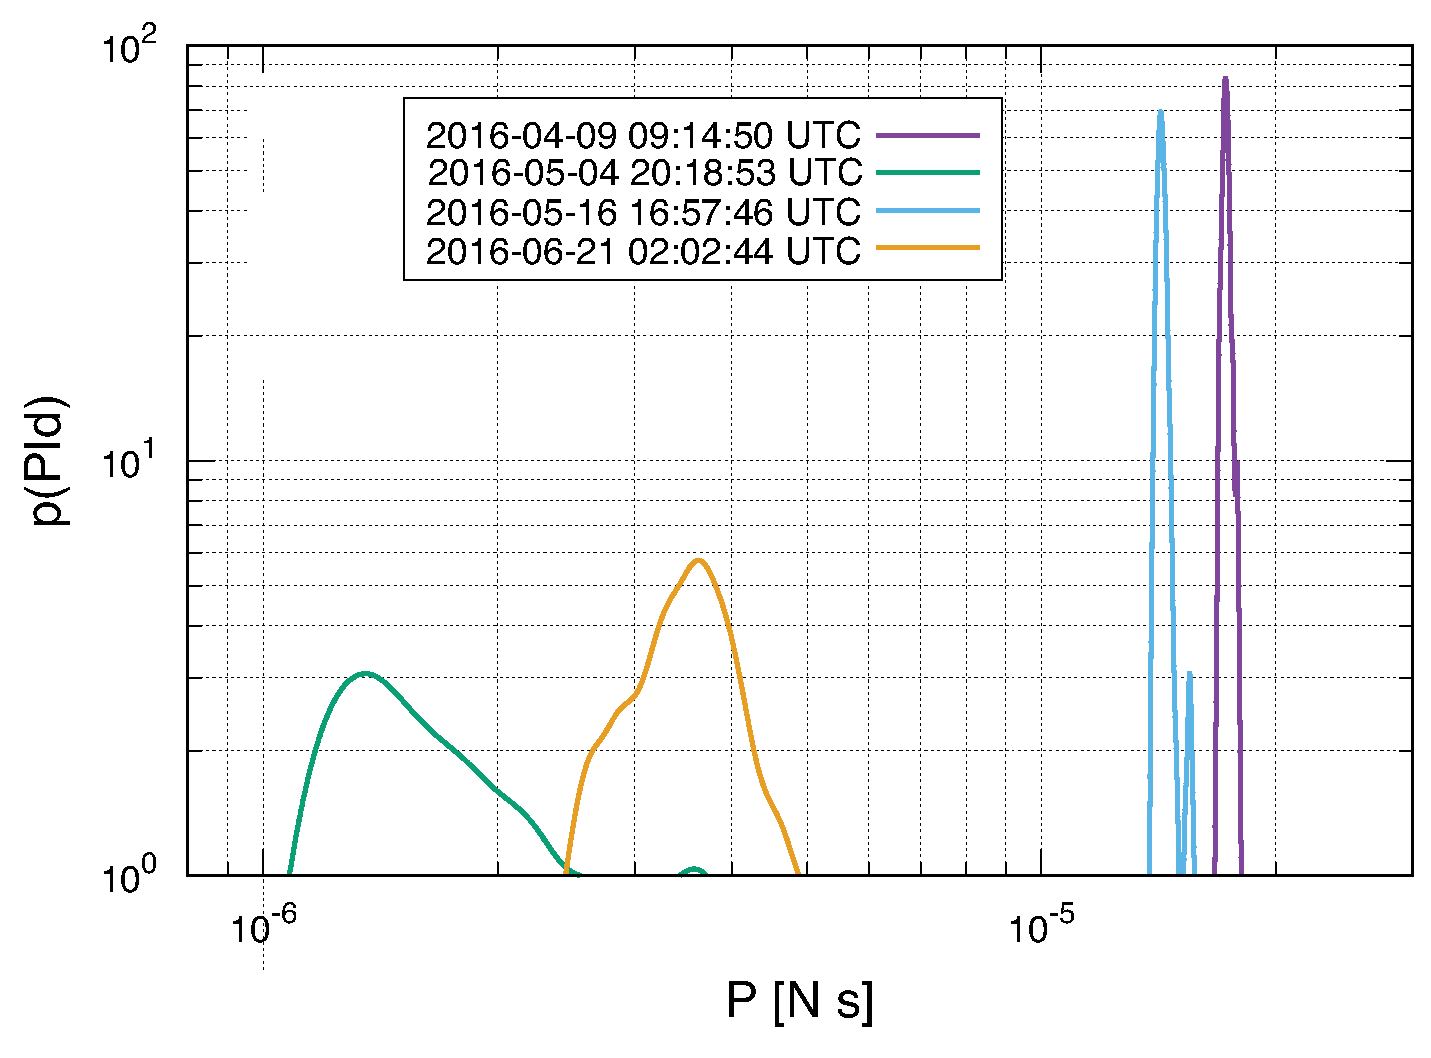
\includegraphics[width=12 cm]{figures/amplitudes.eps}
	\caption{\label{fig:amps}Posterior distribution functions of reconstructed amplitudes for the four example impact candidates.}
\end{figure}
\begin{figure}[h!]
	\centering
	\subfloat[2016-04-09\label{fig:sky1}]{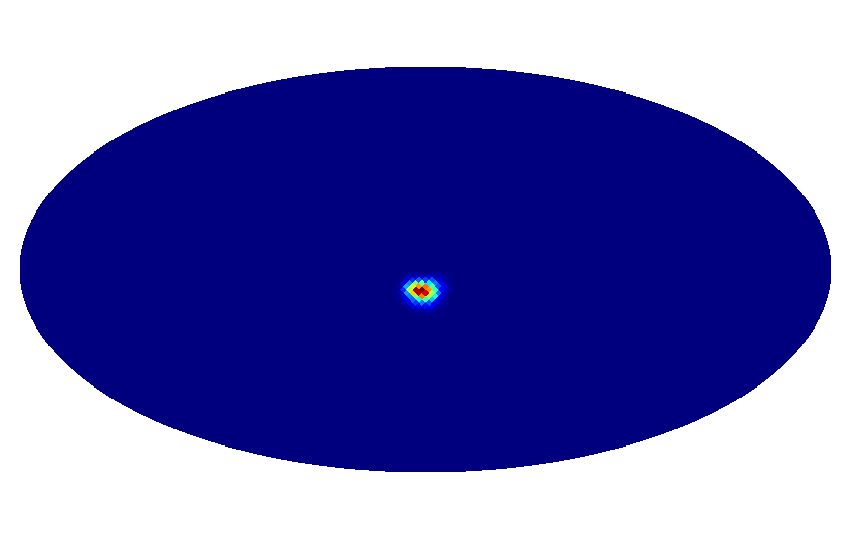
\includegraphics[width=7 cm]{figures/sky1.png}}\quad
	\subfloat[2016-05-04\label{fig:sky2}]{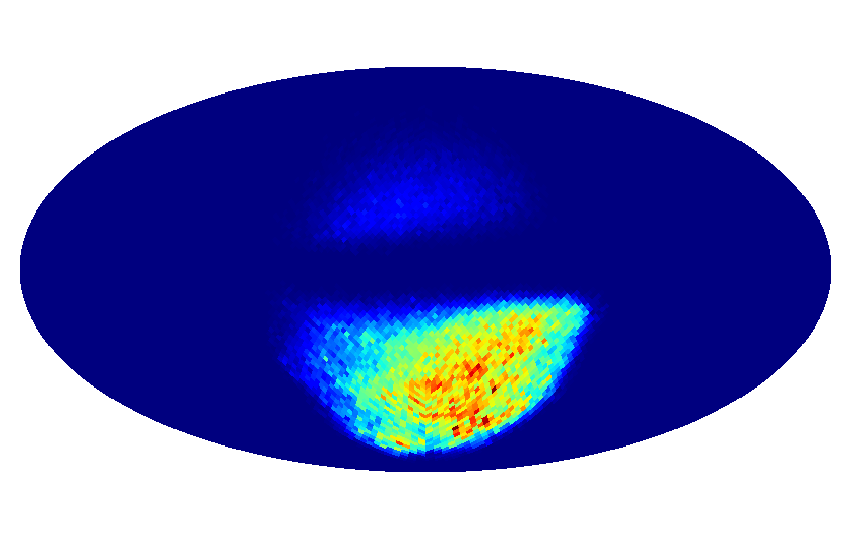
\includegraphics[width=7 cm]{figures/sky2.png}}\\	
        \subfloat[2016-05-16\label{fig:sky3}]{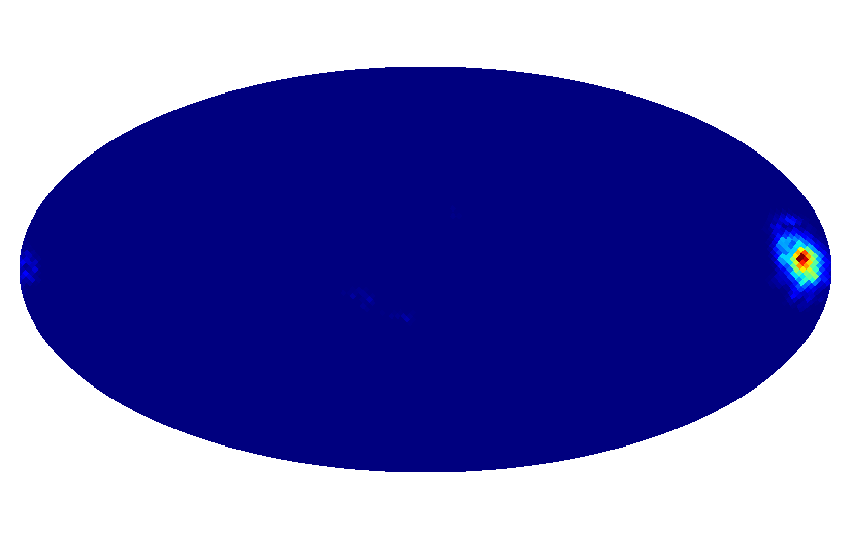
\includegraphics[width=7 cm]{figures/sky3.png}}\quad
	\subfloat[2016-06-21\label{fig:sky4}]{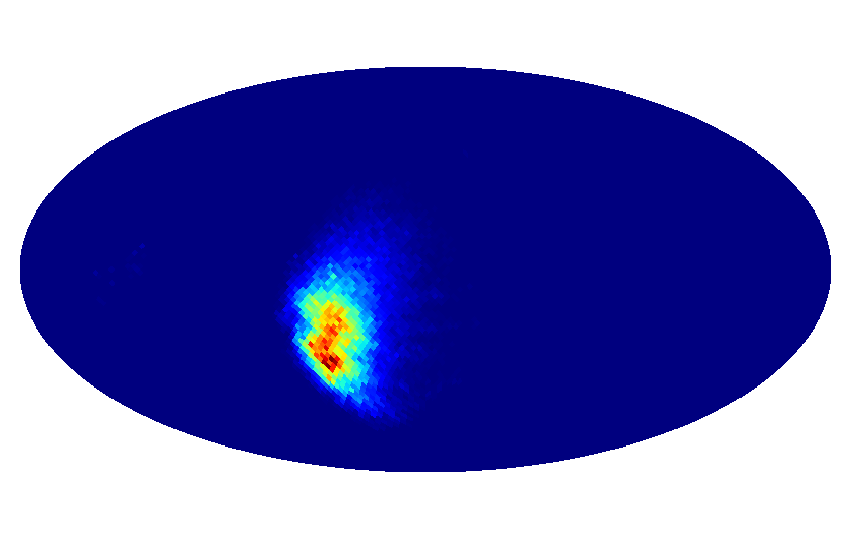
\includegraphics[width=7 cm]{figures/sky4.png}}\\	
	\caption{Reconstructed sky position histograms for the four example impact candidates. Sky maps are Mollweide projections with zero longitude along the $+x$ axis of the SC and $+90^{\circ}$ latitude along the $+z$ direction.}
\end{figure}
\begin{figure}[h!]
	\centering
	\subfloat[2016-04-09\label{fig:loc1}]{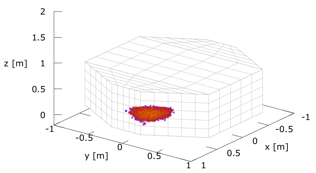
\includegraphics[width=7 cm]{figures/faces1.png}}\quad
	\subfloat[2016-05-04\label{fig:loc2}]{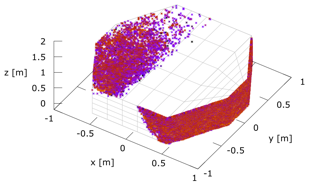
\includegraphics[width=7 cm]{figures/faces2.png}}\\	
        \subfloat[2016-05-16\label{fig:loc3}]{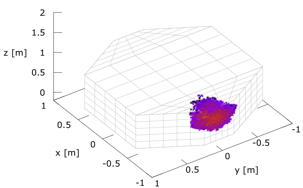
\includegraphics[width=7 cm]{figures/faces3.png}}\quad
	\subfloat[2016-06-21\label{fig:loc4}]{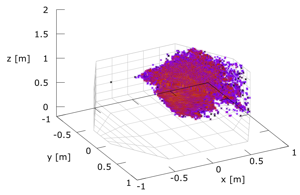
\includegraphics[width=7 cm]{figures/faces4.png}}\\	
	\caption{Reconstructed impact locations for the four example impact candidates. Points are MCMC chain locations after burn-in, color coded by log likelihood with warmer colors representing higher likelihood.}
\end{figure}
\FloatBarrier

\section{Discussion}
\label{sec:discuss}
The impact candidates presented in Section \ref{sec:results} demonstrate that detecting and characterizing impact events with LPF is achievable in practice. However, additional steps are needed before this work is complete. 
\par
First, the impact candidates need to be vetted and vetoed against any possible non-impact transients that fool the search process.  There are two general classes of these transients. The first is a transient in the test mass system, either a force applied on the test mass such as an outgassing event or a sensor glitch. Our approach to guarding against these types of transients will be to utilize both the reference and non-reference test masses aboard LPF to simultaneously search for impact events. Spurious transients of this type will either show up in only one test mass or will be fit with inconsistent parameters between the two test masses.
\par
The second kind of transient is an external force on the spacecraft that is not arising from a micrometeoroid impact. The most likely culprit is one of the two micro-propulsion systems, which may occasionally produce a thrust transient which would by definition be common mode in the two test masses. These transients will be vetoed by comparing the recovered location and sky angles of the impacts with the thruster location and directions as well as by examining  thruster diagnostic signals in the time period around an impact. Other non-impact disturbances are not expected to have the short period impulse in acceleration that is characteristic of an impact. 
\par
Another avenue of research is to compare the number and type of impacts detected with models of the dust environment in the inner solar system. This will require a more complete catalog of events as well as a model that can predict the flux of impacts near L1 as a function of particle mass and velocity. If a sufficient number of events are detected, a detailed comparison of such a model with data can be made, thus using a gravitational wave technology demonstrator to inform our knowledge of the dust environment in the inner solar system.
\section*{References}
\bibliographystyle{iopart-num}
\bibliography{Bibliography}

\end{document}

